\section{Computation of derivatives}
\label{sec:derivatives}

Computation of derivative quantities such as gradient and Laplacian is of fundamental importance in
data analysis. In this section, we study streams that aim to minimize errors of derivative fields.
For the experiments in this section, we quantize the data to $32$ instead of $16$ bits, to ensure
enough precision for the purpose of taking derivatives using finite differences of floating-point
values. Note that in this paper, for the purpose of derivative computation, we always perform finite
differences on the finest (original) resolution. This is possible since the wavelet transform allows
for reconstruction of the function at the original resolution. The reason for this decision is to
avoid the problem of computing distances between quantities across grids of different dimensions
(e.g., computing the root-mean-square error between a (down-sampled) $n\times n$ grid and a
$2n\times 2n$ grid), because we are unaware of solutions to this problem. In the following Sections,
we perform experiments with two of the most common types of derivative, namely gradient and
Laplacian.

\subsection{Gradient}

Since simulation data can rarely be captured by closed-form formulas, we use finite difference to
compute gradients. We experiment with three popular finite difference schemes using stencil size
widths of two, three, and five points in each dimension: $\frac{\partial f}{\partial x}\approx
f(x+1)-f(x)
\approx \frac{1}{2}f(x+1)-\frac{1}{2}f(x-1) \approx
\frac{1}{12}f(x-2)-\frac{2}{3}f(x-1)+\frac{2}{3}f(x+1)-\frac{1}{12}f(x+2)$. In 2D, the gradient at
each grid point $(x,y)$ is the vector $(\frac{\partial f}{\partial x},\frac{\partial f}{\partial
y})$. We use the greedy algorithm in Section (\Cref{sec:data_dep_streams} to compute a
\emph{gradient-optimized} stream that minimizes the difference between the gradient field of $f_b$
(the reconstructed function using $b$ bits per sample) and that of the original function ($f$). At
each grid point $p$, we compute an error $e(p)$, defined to be the squared Euclidean length of the
difference between two gradient vectors at $p$, that is $e(p)=\norm{\nabla f_b(p)-\nabla f(p)}^2$.
The overall error metric over the whole field, $E_g$, is defined as $E_g(\nabla f_b,\nabla
f)=\sqrt{\frac{1}{n}\sum_{i=1}^{n}{e(p_i)}}$.

We first want to quantify the effects (if any) that the stencil width has on the performance of
\emph{gradient-optimized} streams. For this experiment, we treat the gradient computed using the
five-point stencil on the finest resolution grid, at full precision, as the ``groundtruth'' gradient
field. Three \emph{gradient-optimized} streams (2-point, 3-point, and 5-point) are compared against
this groundtruth gradient field, using the error criteria $E_g$ defined above. The results are
plotted in Figure \ref{fig:gradient-stencil-comparison}. The error curves for all three stencils
match one another closely, with the two-point stencil having negligibly higher errors in some cases.
Subsequent experiments in the section uses the five-point stencil always.

\begin{figure}
	\centering
	\subcaptionbox{boiler}
	{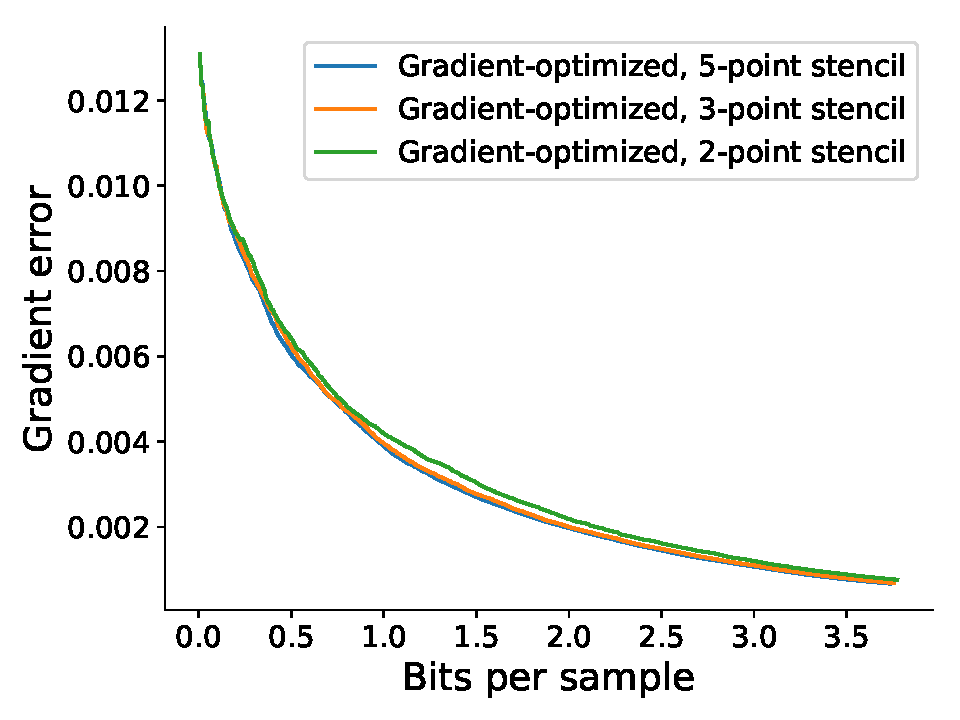
\includegraphics[width=0.48\linewidth]{img/gradient/compare-stencils/gradient-optimized-boiler.pdf}}
	\subcaptionbox{diffusivity}
	{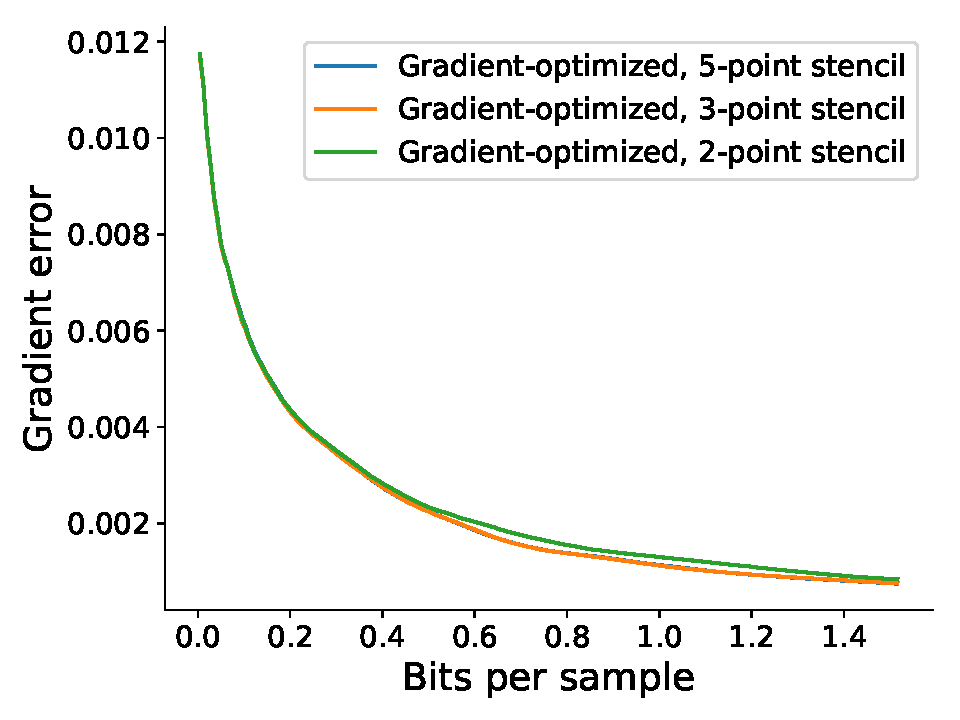
\includegraphics[width=0.48\linewidth]{img/gradient/compare-stencils/gradient-optimized-diffusivity.pdf}}
	\subcaptionbox{euler}
	{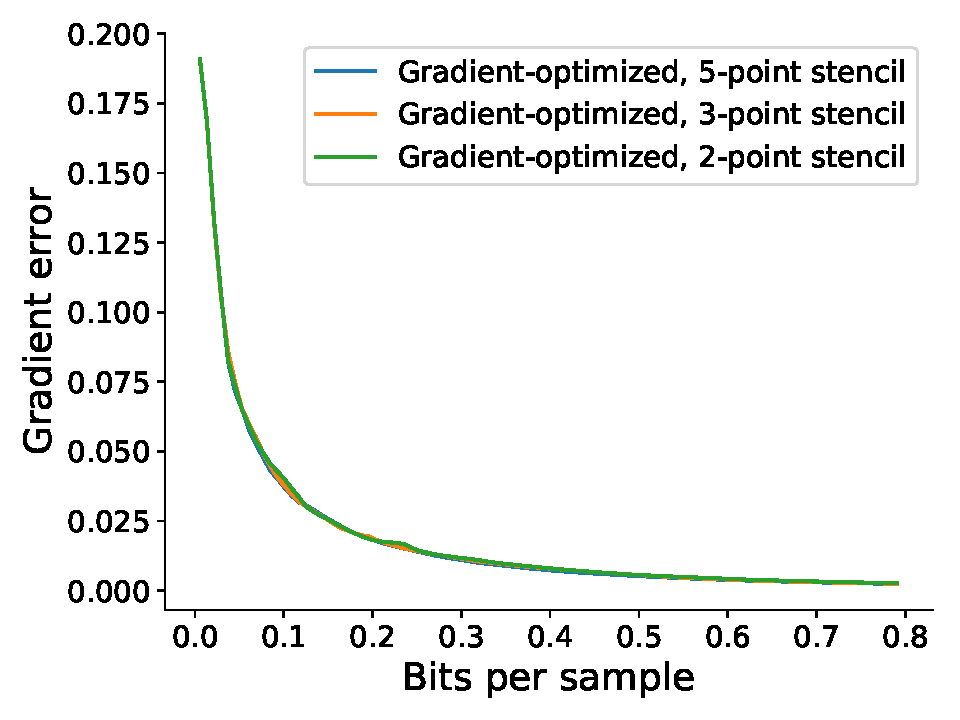
\includegraphics[width=0.48\linewidth]{img/gradient/compare-stencils/gradient-optimized-euler.pdf}}
	\subcaptionbox{pressure}
	{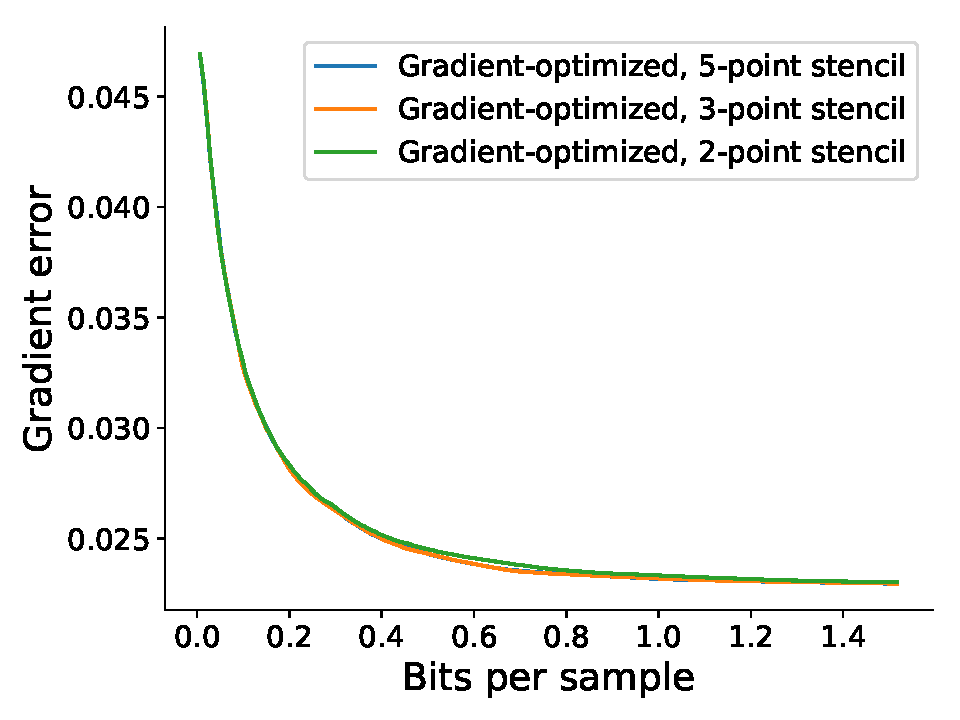
\includegraphics[width=0.48\linewidth]{img/gradient/compare-stencils/gradient-optimized-pressure.pdf}}
	\subcaptionbox{marschner-lobb}
	{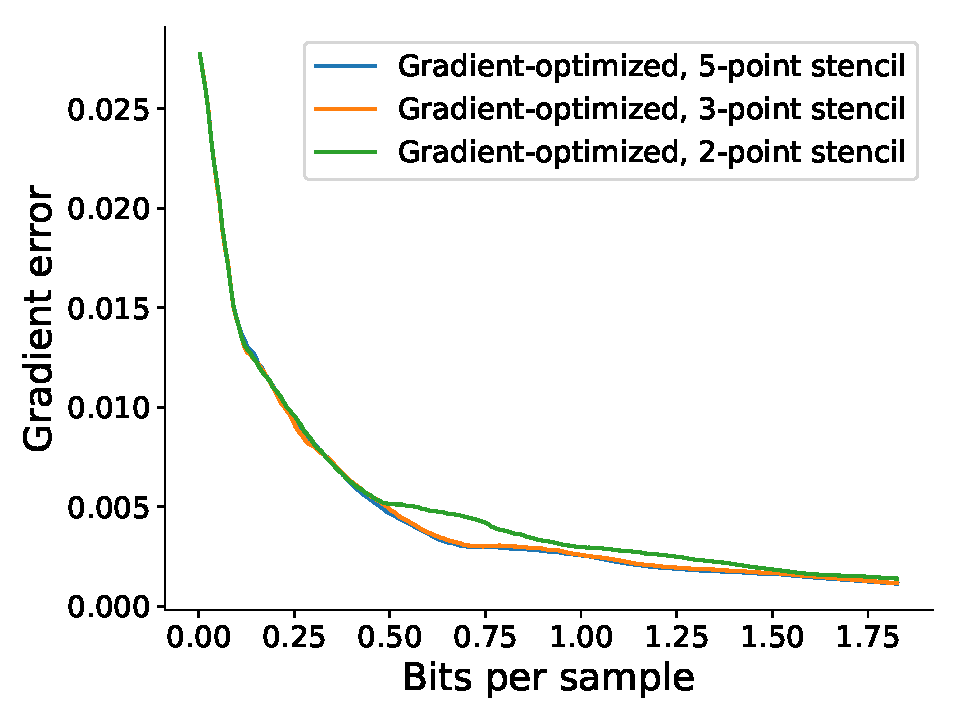
\includegraphics[width=0.48\linewidth]{img/gradient/compare-stencils/gradient-optimized-marschner-lobb.pdf}}
	\subcaptionbox{velocityz}
	{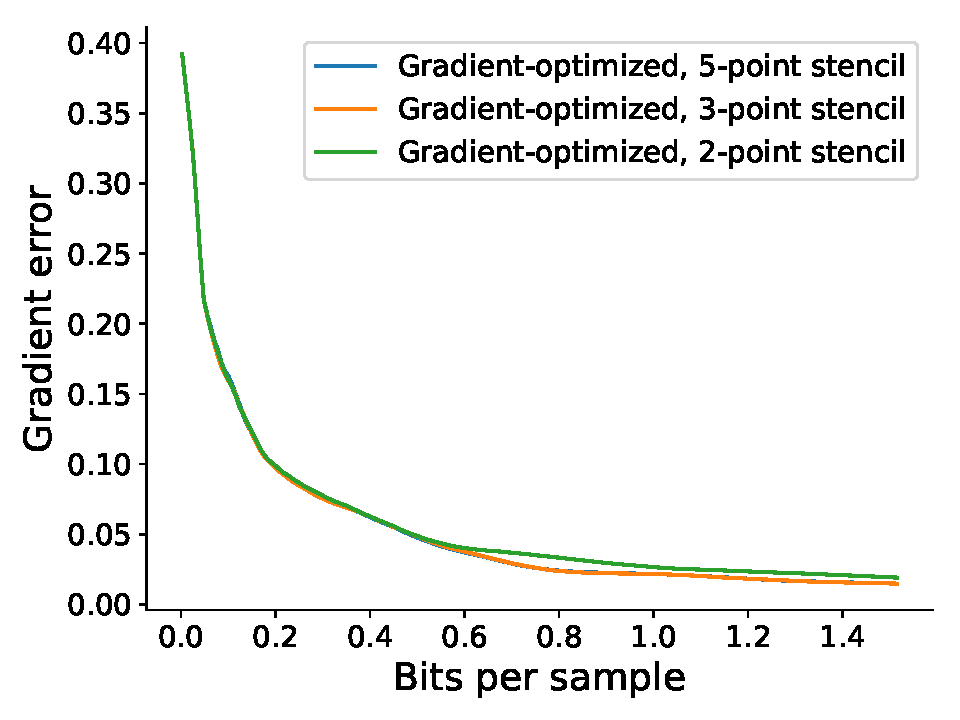
\includegraphics[width=0.48\linewidth]{img/gradient/compare-stencils/gradient-optimized-velocityz.pdf}}
	\caption{Gradient error for \emph{gradient-optimized} streams using different stencil widths,
	againts the ``groundtruth'' gradient, computed using 5-point finite difference on the original
	field. The plots are truncated towards the end, so as to better highlight differences between the
	curves. It can be seen that in most cases, there are no meaningful differences among the different
	stencil widths. The largest difference in error happens at 0.67 bps, for \emph{marschner-lobb}, in
	which the two-point scheme produces, on average, an error vector that is four-third longer than
	ones produced by the other two.}
	\label{fig:gradient-stencil-comparison}
\end{figure}

In the next experiment, we plot the gradient error curves produced by \emph{gradient-optimized},
together with ones produced by the \emph{by level}, \emph{by bit plane}, and \emph{by wavelet norm}
streams, for the same six data sets. These curves are plotted in Figure
\ref{fig:gradient-error-comparison}. As can be seen from the Figure, \emph{gradient-optimized}
typically performs far better than the data-independent streams, due to the fact that
\emph{gradient-optimized}, with the knowledge of the data, is able to better prioritize regions that
would benefit the most from additional bits. Among the data-independent streams, \emph{by level}
performs the worst, while \emph{by wavelet norm} performs slightly worse than the other two streams,
but the differences in most cases are negligible.

In Figure \ref{fig:gradient-rendering} we visualize the three reconstructed, as well as the
groundtruth, gradient fields for the \emph{marschner-lobb} data set, at 0.52 bps, which is the only
case (among all the tested bit rates and data sets) in which the visualized gradient fields show
noticable differences. It is arguable that the differences are small, and would largely vanish at a
slightly higher bit rate (e.g., 0.6 bps). For this reason, in practice, the best stream to use would
likely be \emph{by bit plane}, due to \emph{gradient signature} being a lot more expensive to
compute in comparison. Otherwise, \emph{by wavelet norm} is a reasonable alternative, especially if
the bits are stored on disk in the same order, to optimize for root-mean-square errors (see Section
\ref{sec:motivation}, for example.

\begin{figure}
	\centering
	\subcaptionbox{boiler}
	{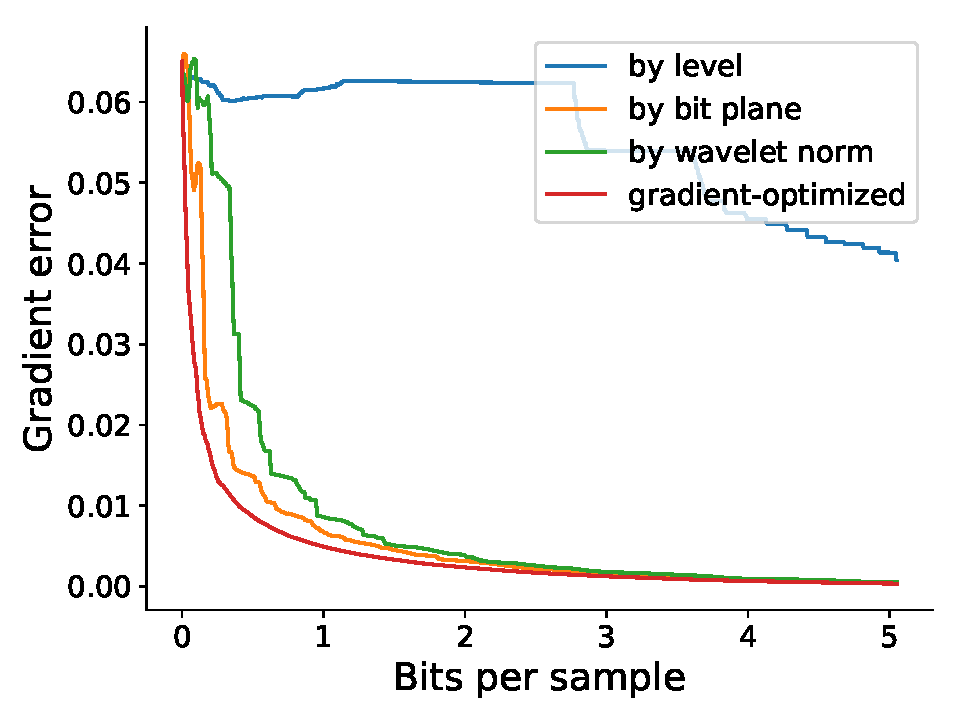
\includegraphics[width=0.48\linewidth]{img/gradient/5points/gradient-optimized-boiler.pdf}}
	\subcaptionbox{diffusivity}
	{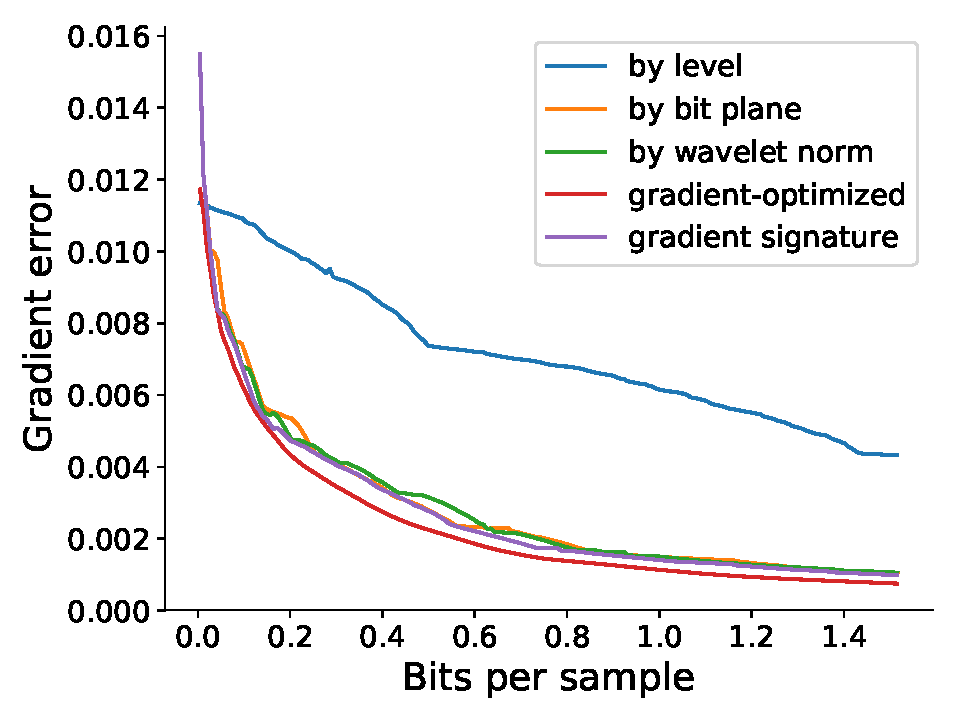
\includegraphics[width=0.48\linewidth]{img/gradient/5points/gradient-optimized-diffusivity.pdf}}
	\subcaptionbox{euler}
	{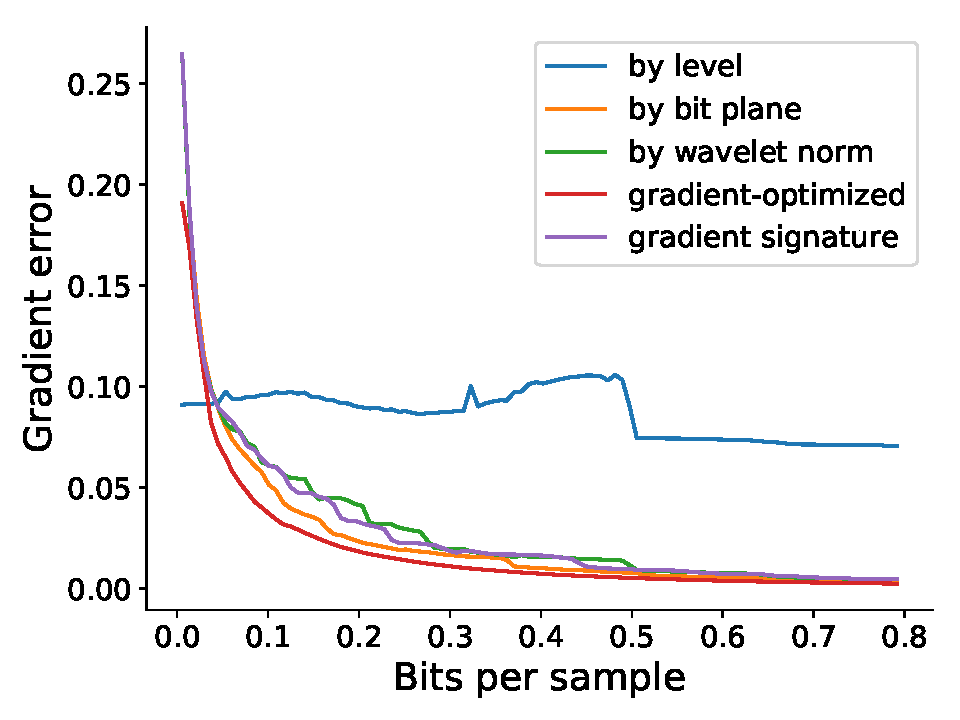
\includegraphics[width=0.48\linewidth]{img/gradient/5points/gradient-optimized-euler.pdf}}
	\subcaptionbox{pressure}
	{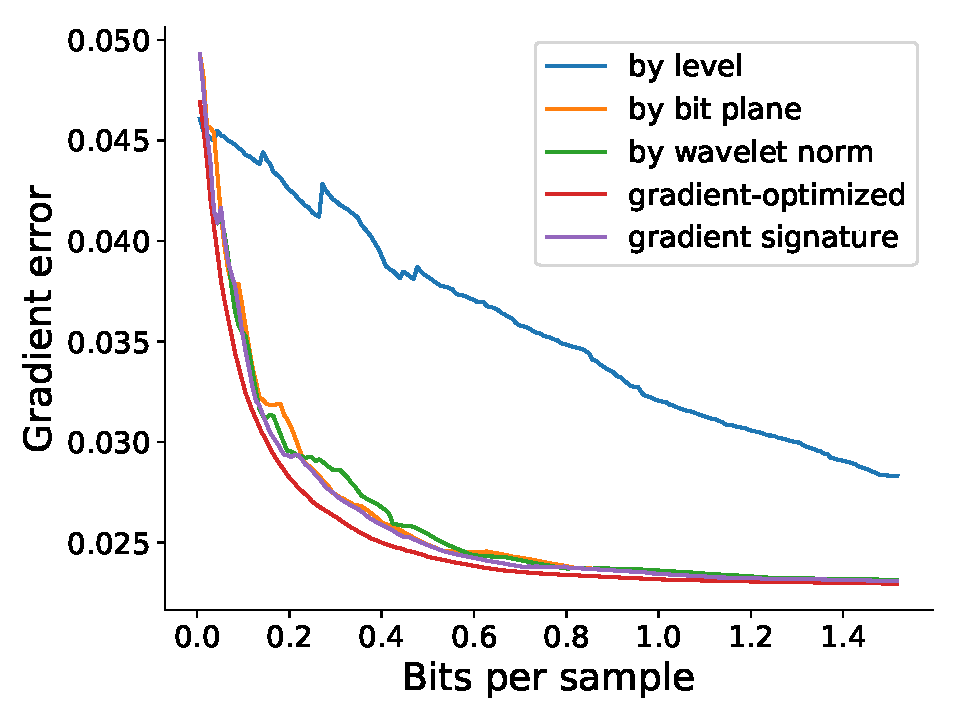
\includegraphics[width=0.48\linewidth]{img/gradient/5points/gradient-optimized-pressure.pdf}}
	\subcaptionbox{marschner-lobb}
	{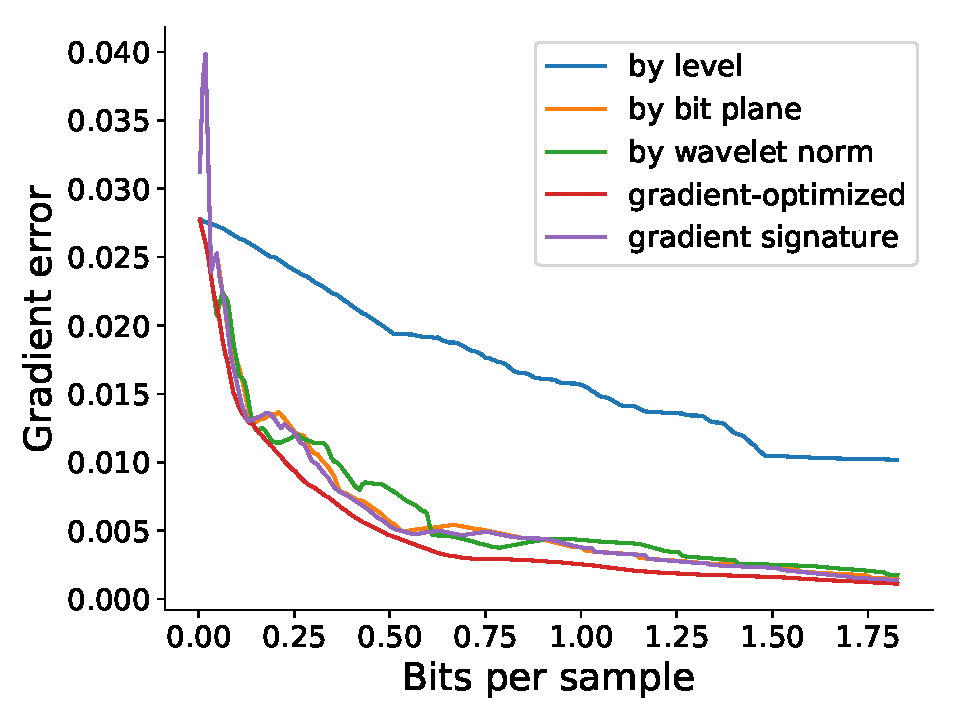
\includegraphics[width=0.48\linewidth]{img/gradient/5points/gradient-optimized-marschner-lobb.pdf}}
	\subcaptionbox{velocityz}
	{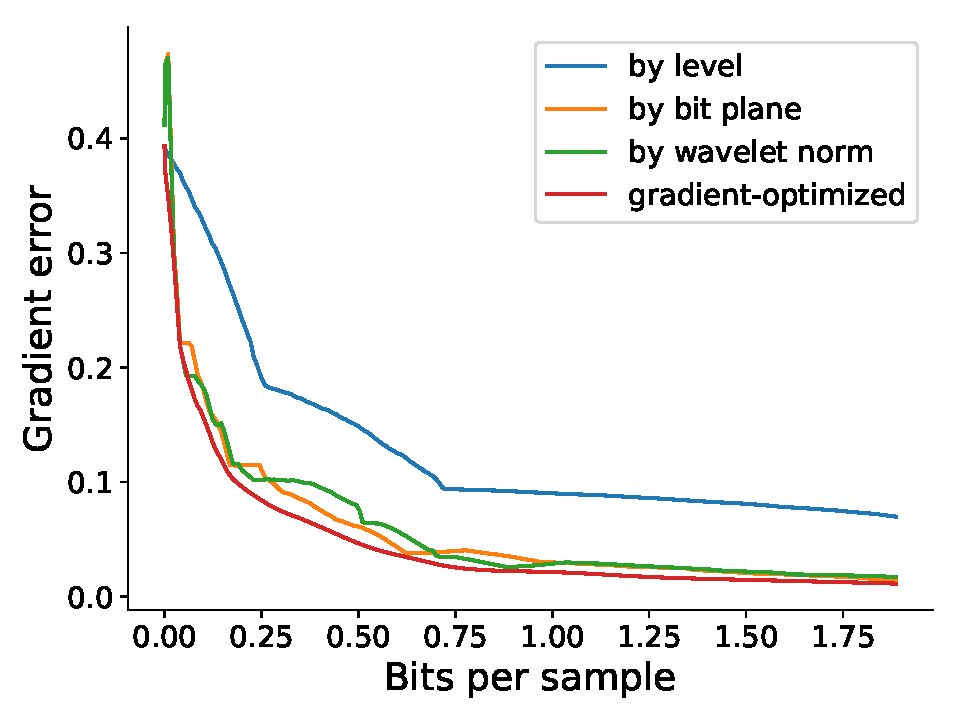
\includegraphics[width=0.48\linewidth]{img/gradient/5points/gradient-optimized-velocityz.pdf}}
	\caption{Gradient error comparison among \emph{gradient-optimized}, \emph{rmse-optimized},
	\emph{by wavelet norm}, and \emph{gradient signature} streams, using the five-point stencil. The
	plots are truncated in the same way as in Figure \ref{fig:gradient-stencil-comparison}. In all
	cases, \emph{by wavelet norm} performs slightly worse than \emph{by bit plane} and \emph{gradient
	signature} do, but the differences are largely negligible. \emph{by level} performs the worst.}
	\label{fig:gradient-error-comparison}
\end{figure}

\begin{figure}
	\centering
	\subcaptionbox{by wavelet norm}
	{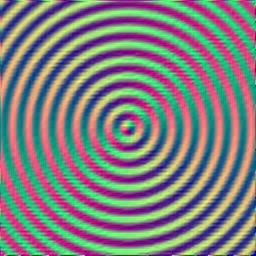
\includegraphics[width=0.49\linewidth]{img/gradient/gradient_0.png}}
	\subcaptionbox{by bit plane}
	{
\includegraphics[width=0.49\linewidth]{img/gradient/gradient_1.png}}
	\subcaptionbox{gradient signature}
	{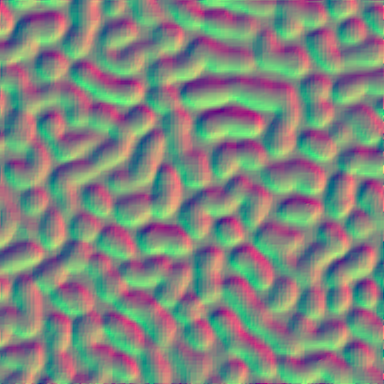
\includegraphics[width=0.49\linewidth]{img/gradient/gradient_2.png}}
	\subcaptionbox{groundtruth}
	{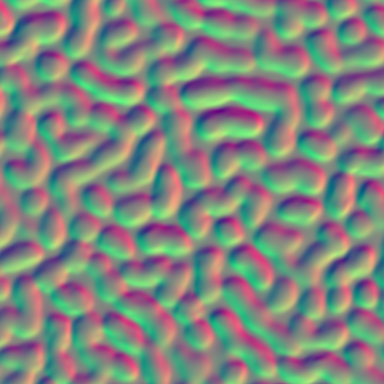
\includegraphics[width=0.49\linewidth]{img/gradient/groundtruth_gradient_0.png}}
	\caption{Comparison of reconstructed gradient fields among \emph{by wavelet norm}, \emph{by bit
	plane} and \emph{gradient signature} streams, for the \emph{marschner-lobb} function, at 0.52 bps.
	The \emph{by bit plane} and \emph{gradient signature} stream produce gradient fields with fewer
	artifacts (see the lower-left corners of the images, for example). }
  \label{fig:gradient-rendering}
\end{figure}

\subsection{Laplacian}

For Laplacian, we use the three-point finite difference in each dimension separately:
$\frac{{\partial}^2}{\partial{x^2}}f(x,y) \approx f(x-1,y)-2f(x,y)+f(x+1,y)$, and $\Delta
f=(\frac{{\partial}^2}{\partial{x^2}}+\frac{{\partial}^2}{\partial{y^2}})f$. The Laplacian error is
defined as the RMSE between the reconstructed Laplacian scalar field and the original Laplacian
scalar field. Again, algorithm [REF] is used to compute a \emph{laplacian-optimized} bit stream that
minimizes this error. In Figure \ref{fig:laplacian-comparison} we compare this stream with the
\emph{rmse-optimized} stream using the PSNR of the difference in Laplacian (compared to the
ground truth) as the error metric. The stream labeled \emph{laplacian signature} is to be ignored for
now. (TODO: why is it in the plot? maybe do not mention it at all? or just say that it will be explained later)

\begin{figure}
	\centering
	\subcaptionbox{boiler, 5-point stencil}
	{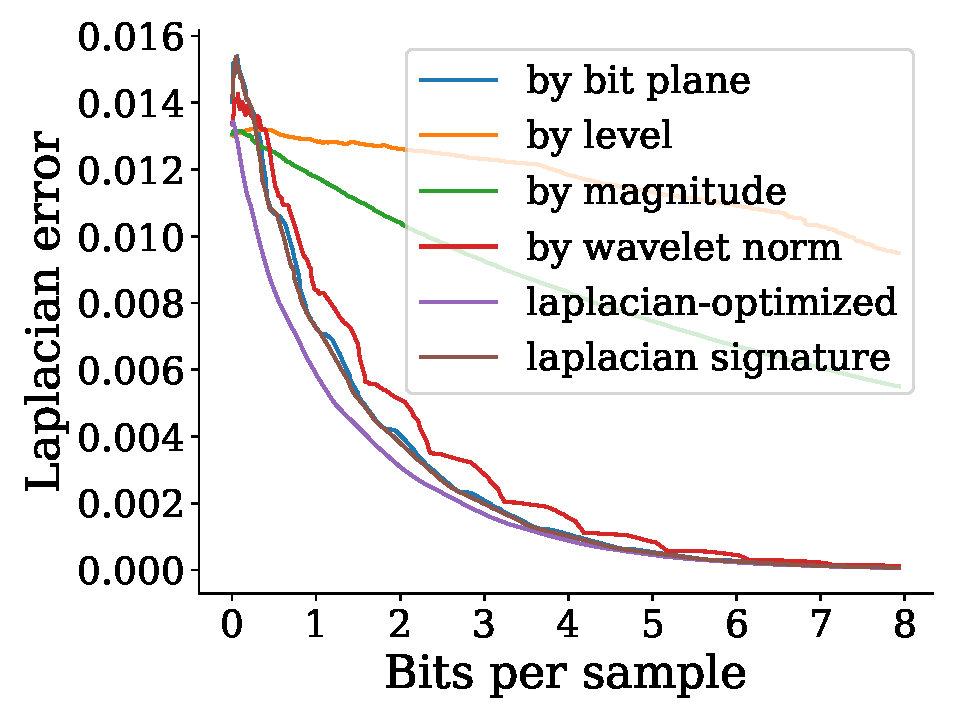
\includegraphics[width=0.48\linewidth]{img/laplacian/laplacian-optimized-boiler.pdf}}
	\subcaptionbox{diffusivity, 5-point stencil}
	{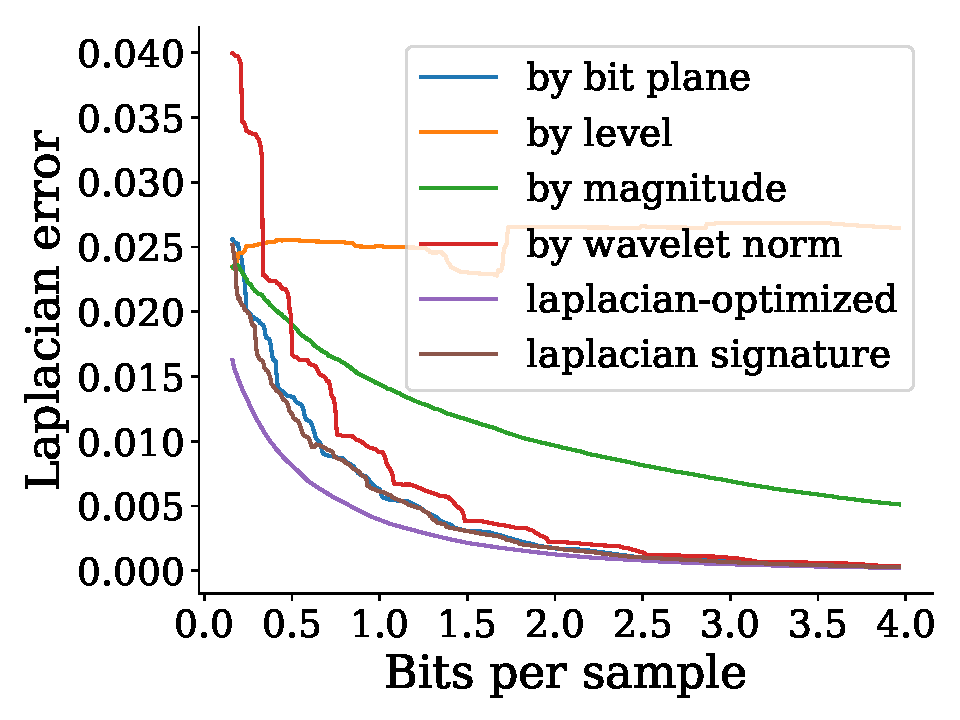
\includegraphics[width=0.48\linewidth]{img/laplacian/laplacian-optimized-diffusivity.pdf}}
	\subcaptionbox{euler, 5-point stencil}
	{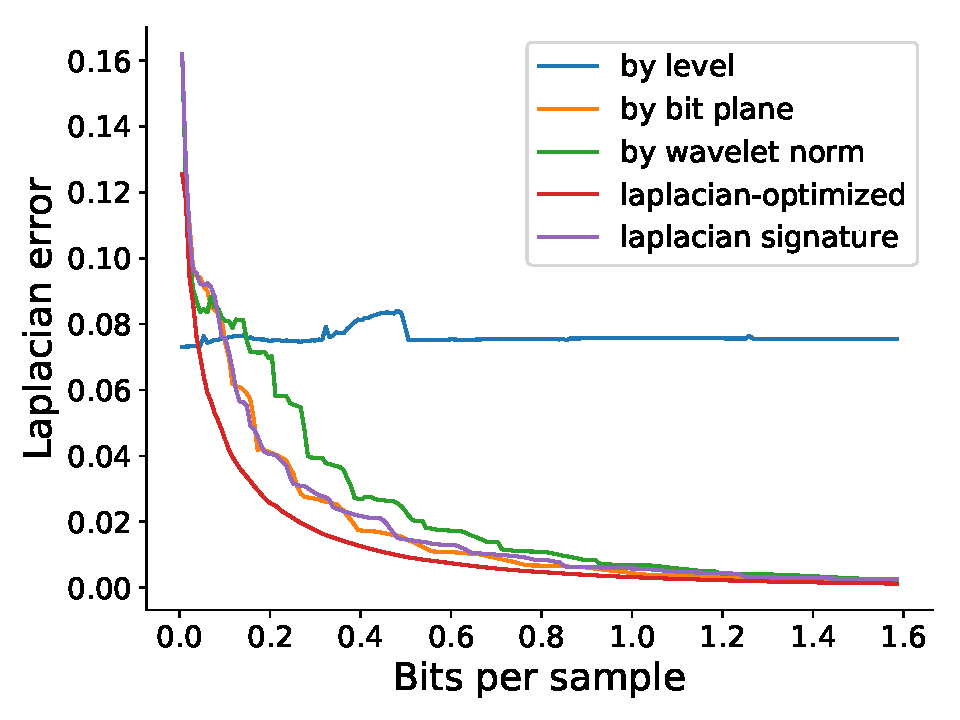
\includegraphics[width=0.48\linewidth]{img/laplacian/laplacian-optimized-euler.pdf}}
	\subcaptionbox{pressure, 5-point stencil}
	{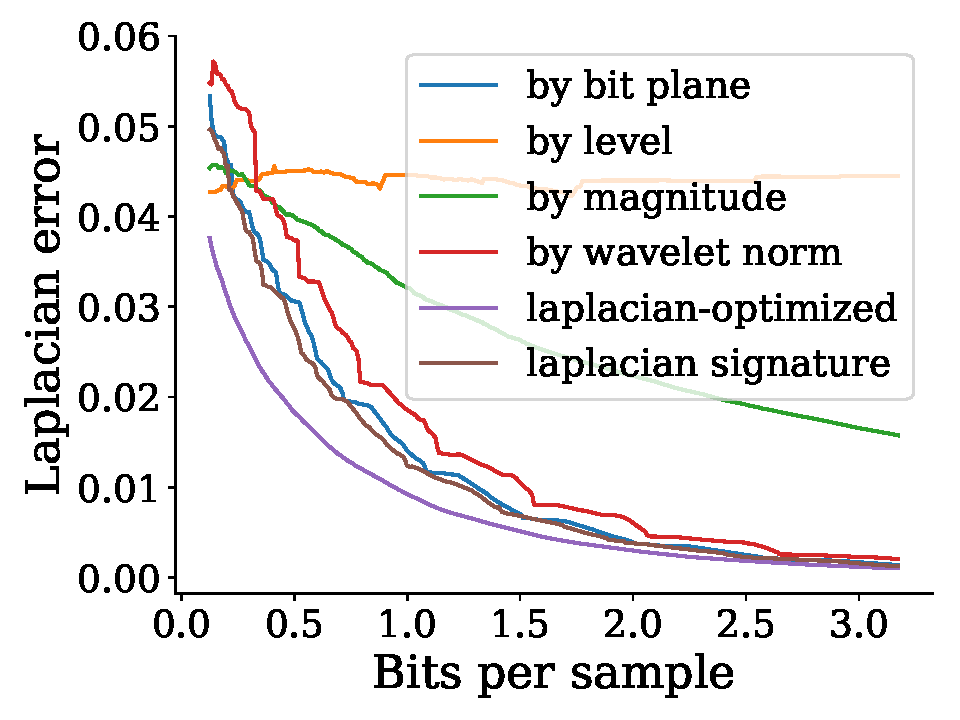
\includegraphics[width=0.48\linewidth]{img/laplacian/laplacian-optimized-pressure.pdf}}
	\subcaptionbox{marschner-lobb, 5-point stencil}
	{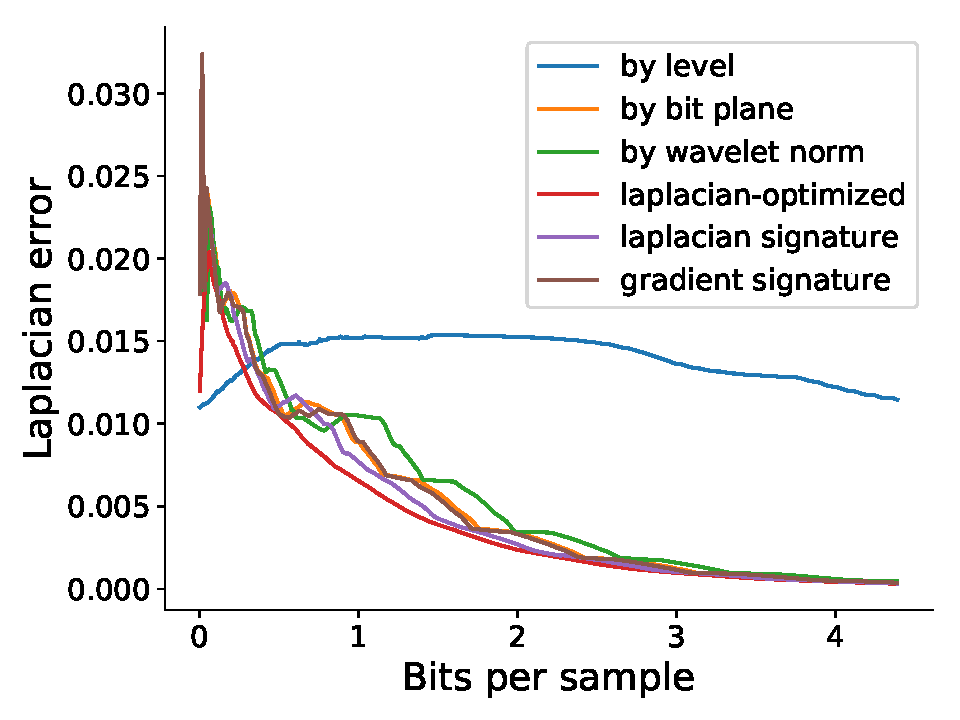
\includegraphics[width=0.48\linewidth]{img/laplacian/laplacian-optimized-marschner-lobb.pdf}}
	\subcaptionbox{velocityz, 5-point stencil}
	{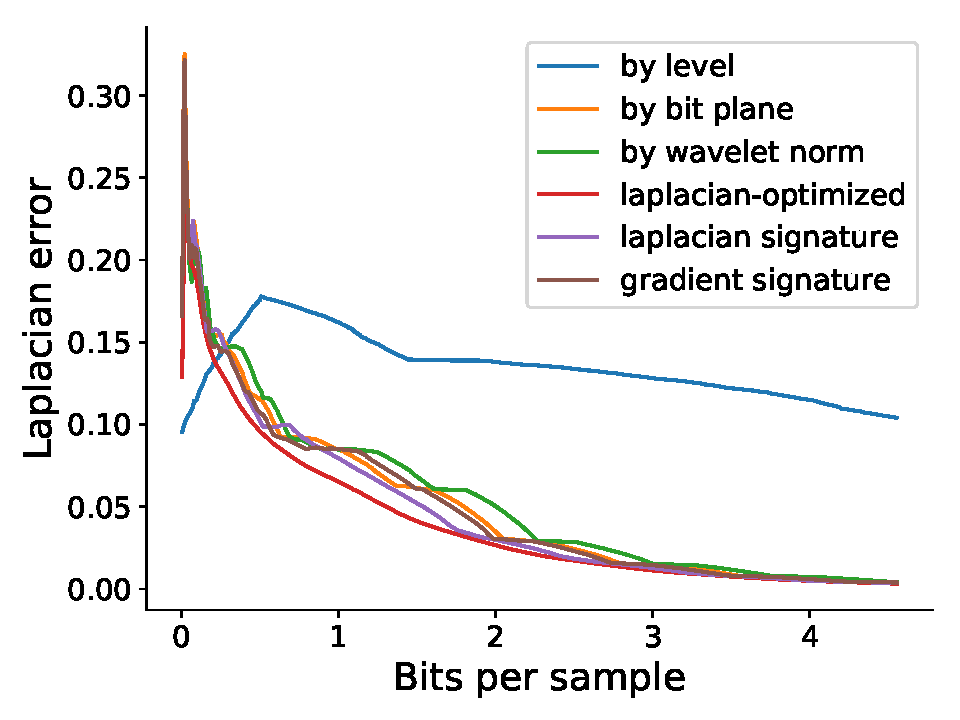
\includegraphics[width=0.48\linewidth]{img/laplacian/laplacian-optimized-velocityz.pdf}}
	\caption{Laplacian error}
	\label{fig:gradient-error-comparison}
\end{figure}

It can be observed that unlike the case for gradient, there exists significant differences between
the \emph{rmse-optimized} and \emph{laplacian-optimized} streams with regards. To understand these
differences we plot the precision of every wavelet coefficients at a low bit rate in Figure
\ref{fig:laplacian-precision-comparison} (a and b). When cross refererencing this Figure with Figure
\ref{fig:gradient-comparison}b we see that the \emph{laplacian-optimized} stream priotizes
finer-resolution bits where the sharp shockwave is, unlike the \emph{rmse-optimized} stream which
prefers lower-ordered, coarse-resolution bits. This effect makes sense intuitively, as the
derivative operator makes functions less smooth, hence amplifing hard edges. This happens in the
gradient case too, but to a much lesser degree.

\begin{figure}
	\centering
	\subcaptionbox{\emph{by wavelet norm}}
	{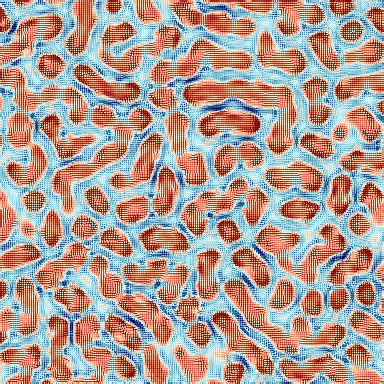
\includegraphics[width=0.48\linewidth]{img/laplacian/laplacian_0.png}}
	\subcaptionbox{\emph{by bit plane}}
	{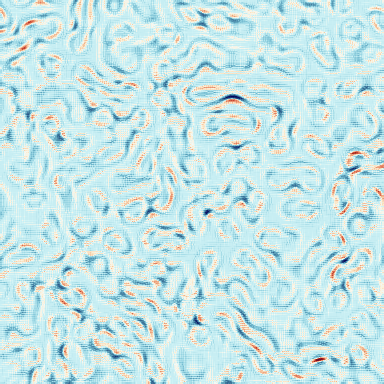
\includegraphics[width=0.48\linewidth]{img/laplacian/laplacian_1.png}}
	\subcaptionbox{\emph{laplacian signature}}
	{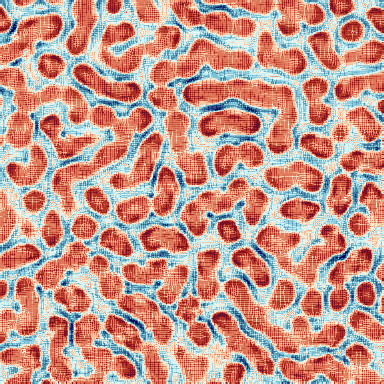
\includegraphics[width=0.48\linewidth]{img/laplacian/laplacian_2.png}}
	\subcaptionbox{\emph{groundtruth}}
	{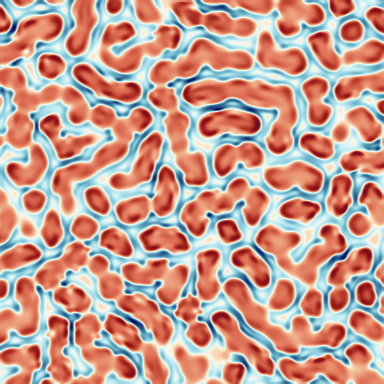
\includegraphics[width=0.48\linewidth]{img/laplacian/groundtruth_laplacian_0.png}}
	\caption{Laplacian rendering, diffusivity}
	\label{fig:laplacian-precision-comparison}
\end{figure}

\begin{figure}
	\centering
	\subcaptionbox{\emph{by wavelet norm}}
	{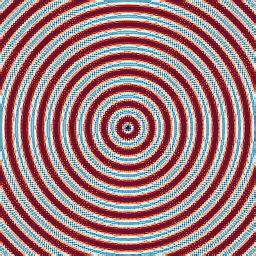
\includegraphics[width=0.48\linewidth]{img/laplacian/laplacian_00.png}}
	\subcaptionbox{\emph{by bit plane}}
	{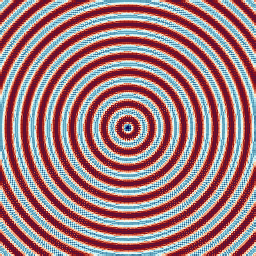
\includegraphics[width=0.48\linewidth]{img/laplacian/laplacian_11.png}}
	\subcaptionbox{\emph{laplacian signature}}
	{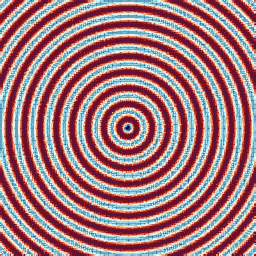
\includegraphics[width=0.48\linewidth]{img/laplacian/laplacian_22.png}}
	\subcaptionbox{\emph{groundtruth}}
	{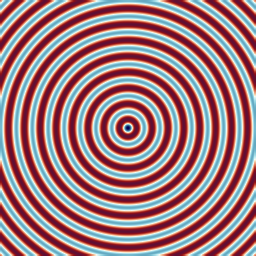
\includegraphics[width=0.48\linewidth]{img/laplacian/groundtruth_laplacian_00.png}}
	\caption{Laplacian rendering, marschner-lobb}
	\label{fig:laplacian-precision-comparison}
\end{figure}

\begin{figure}
	\centering
	\subcaptionbox{\emph{laplacian-optimized}}
	{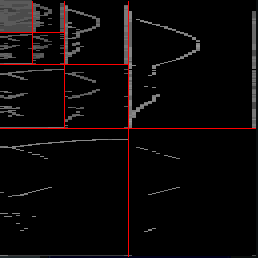
\includegraphics[width=0.32\linewidth]{img/gradient-laplacian/euler-prec-lap.png}}
	\subcaptionbox{\emph{rmse-optimized}}
	{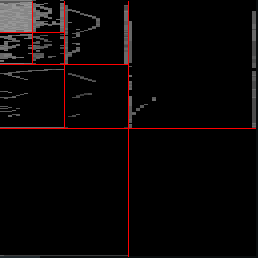
\includegraphics[width=0.32\linewidth]{img/gradient-laplacian/euler-prec-rmse.png}}
	\subcaptionbox{\emph{laplacian signature}}
	{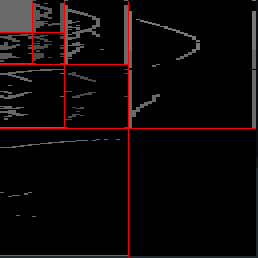
\includegraphics[width=0.32\linewidth]{img/gradient-laplacian/euler-prec-signature.png}}
	\caption{Precision distribution of wavelet coefficients at 0.25 bits per sample for the euler data
	set. Each square box with red boundary is a wavelet subband (the coarsest subband is in the top
	left). Brighter pixels correspond to higher-precision wavelet coefficients (black means no bit of
	that coefficient has not been received, while white means the whole coefficient has been
	received).}
	\label{fig:laplacian-precision-comparison}
\end{figure}

\emph{rmse-optimized}, \emph{laplacian-optimized}, and also \emph{gradient-optimized} for the euler
data set are visualized in Figure \ref{fig:signature-comparison}. 

\begin{figure}
	\centering
	\subcaptionbox{\emph{rmse-optimized}}
	{
\includegraphics[width=0.32\linewidth]{img/gradient-laplacian/SIG-GREEDY-(rmse).png}}
	\subcaptionbox{\emph{laplacian-optimized}}
	{
\includegraphics[width=0.32\linewidth]{img/gradient-laplacian/SIG-GREEDY-(laplacian).png}}
	\subcaptionbox{\emph{gradient-optimized}}
	{
\includegraphics[width=0.32\linewidth]{img/gradient-laplacian/SIG-GREEDY-(gradient).png}}
	\caption{Stream signatures visualized through a linear-blue color map (brighter is higher
	priority). From left to right: higher-ordered to lower-ordered bit planes. From top to bottom:
	coarser to finer subbands. Note that the streams from which the signatures are extracted do not
	contain leading zero bits, which explains the very dark cells }
	\label{fig:signature-comparison}
\end{figure}

Using the signature for \emph{laplacian-optimized}, we are able construct a data-independent stream
(in the sense that once the signature is computed and is given, the ordering of the bits follows the
the signature only). This stream, called \emph{laplacian signature}, performs at least as well as,
and often better, than \emph{rmse-optimized} for all data sets (see Figure
\ref{fig:laplacian-comparison}). The reason \emph{laplacian signature} does not always outperform
\emph{rmse-optimized}, and that there is still a gap between itself and \emph{laplacian-optimized}
is that the signature is computed essentially by `'averaging'' local signatures, a process that
lessen the effectiveness of the signature when the data is highly inhomogenous (e.g., the euler data
set with its sharp shockwaves). Nevertheless, even with one signature for the whole domain, we are
able to reconstruct more accurate Laplacian in all cases in experiment. In practice, the signature
is a tiny piece of meta information that can be pre-computed, stored, and transmitted before any
value bits to help `'steer'' the data stream, whenever Laplacian is the quantity of interest.
